\documentclass[a4paper]{article}

\usepackage[utf8]{inputenc}
\usepackage[portuges]{babel}
\usepackage{indentfirst}
\usepackage{graphicx}
\usepackage{float}
\usepackage{caption}
\usepackage{subcaption}
\usepackage[T1]{fontenc}
\usepackage{listings}
\usepackage{amsmath}
\usepackage{mathtools}
\renewcommand{\familydefault}{\sfdefault}


\title{Projeto de Computação Gráfica - Fase 3}
\author{Diogo Braga A82547 \and João Silva A82005 \and Ricardo Caçador A81064
\and Ricardo Veloso A81919}
\date{\today}

\begin{document}

\maketitle

\begin{abstract}
Neste relatório é apresentada a terceira fase dum projeto no qual a intenção é desenvolver um mecanismo baseado em gráficos 3D e fornecer exemplos de uso que mostrem o seu potencial. Este projeto é desenvolvido no âmbito da unidade curricular de Computação Gráfica.
\end{abstract}


\newpage

\tableofcontents


\newpage

\section{Introdução}
\label{sec:intro}

Nesta terceira fase serão implementadas algumas funcionalidades tanto no \textit{Generator} como no \textit{Engine}, sendo estas:

\begin{enumerate}
\item Ler um ficheiro \textit{patch} que irá conter os pontos de controlo de \textbf{Bezier} e criar o modelo respetivo (cometa).
\item Aprofundar as \textbf{translações} e as \textbf{rotações} alterando o ficheiro "XML" e o seu \textit{parsing}.
  \begin{enumerate}
  \item As \textbf{translações} contendo os pontos de controlo que irão definir uma \textit{Catmull-Rom Cubic Curve} bem como uma variável \textit{time} que representa o tempo (em segundos) que demora a percorrer a curva.
  \item As \textbf{rotações} poderão ter o seu ângulo substituido por tempo sendo este o tempo que demora a realizar um rotação de 360º.
  \end{enumerate}
\item Desenhar os modelos utilizando VBOs aumentado assim a perfomance.
\end{enumerate}

De seguida iremos apresentar figuras, algoritmos e as suas respetivas explicações de forma a ilustrar a realização das etapas apresentadas acima.

\newpage

\section{Estrutura da Pasta do Projeto}
\label{sec:estrutura}

Para um entendimento mais claro da estrutura do projeto, achamos por bem referenciar a estrutura da pasta do projeto.
O projeto entregue contêm para além do relatório, 4 pastas como é possível verificar na seguinte figura.

\begin{figure}[H]
\centering
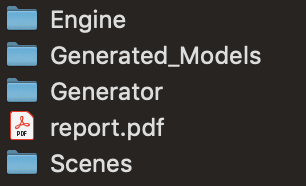
\includegraphics[scale=1.0]{estrutura.png}
\caption{Estrutura da pasta.}
\label{img:estrutura}
\end{figure}

Na pasta \textbf{Engine} residem os ficheiros relativos ao programa \emph{engine}, bem como as bibliotecas (.h) criadas para o efeito. Contém ainda um ficheiro de configuração \emph{cmake} e os ficheiros relativos à biblioteca \emph{tinyxml2}.

Na pasta \textbf{Generator} residem os ficheiros relativos ao programa \emph{generator}. Contém também um ficheiro de configuração \emph{cmake}. Em relação à fase anterior acrescenta a existência de um ficheiro .cpp que irá servir como um parser para o ficheiro \textit{patch} presente na pasta \textbf{Generated\_Models}.

Na pasta \textbf{Generated\_Models} residem os ficheiros que contêm os pontos gerados para cada figura, criados pelo programa \emph{generator}. Relativamente à fase anterior acrescenta a existência de um ficheiro \textit{patch} que irá conter os pontos de controlo.

Na pasta \textbf{Scenes} reside um ficheiro \emph{XML} que contem a estrutura do sistema solar desenvolvido para esta fase do projeto.

\newpage

\section{Parser XML}
\label{sec:parser}

\subsection{Ficheiro}
\label{sec:ficheiro}

Devido aos requerimentos desta fase foi necessário alterar o ficheiro XML que provinha da segunda fase. As alterações aconteceram devido, por exemplo, à necessidade de incluir no ficheiro os pontos de controlo que, mais tarde gerados, dariam como resultado a curva de Catmull-Rom.

Importante referir que também nesta fase todos os sub-grupos herdam as transformações geométricas presentes no grupo ao qual pertencem. Nesta fase, estas transformações são: translações, rotações e escalas.

As escalas mantêm o mesmo funcionamento da fase anterior. Por outro lado, as translações e as rotações têm funcionamentos diferentes.

As translações funcionam tendo em conta um conjunto de 8 pontos que define uma curva de Catmull-Rom, e uma compontente \textit{time} que define o tempo que o objeto demora a realizar a curva. No caso das rotações, estas podem estabelecer o ângulo através da componente habitual \textit{angle}, ou através da componente \textit{time}.

Na figura \ref{img:ficheiro_parser} é possível visualizar um excerto do ficheiro XML referente à Terra e à Lua.

\begin{figure}[H]
\centering
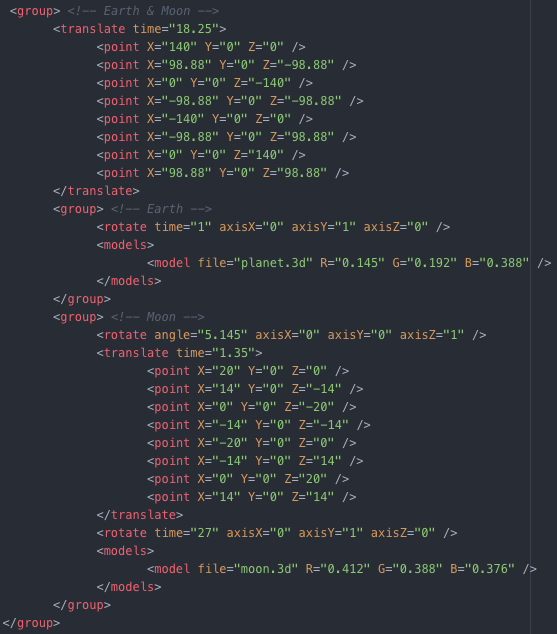
\includegraphics[scale=0.50]{ficheiro_parser.png}
\caption{Exemplo dum ficheiro usado no Parser.}
\label{img:ficheiro_parser}
\end{figure}

\subsection{Funcionamento}
\label{sec:funcionamento}

Tendo em conta as alterações referidas no ponto anterior modificamos também o funcionamento do \textit{parser}.

\ttfamily
\begin{enumerate}
  \item Executa a função "parser\_XML" que abre o ficheiro "scene.xml" e verifica se a leitura foi correta.
  \item Caso se verifique inicia a função "parseGroup".
  \item Nesta função alteramos o funcionamento para o caso do elemento \textit{child} seja uma rotação ou uma translação.
  \item Caso seja uma translação:
  \begin{enumerate}
    \item Obtém o valor \textit{time} e atribui-o à figura.
    \item De seguida itera sobre os 8 pontos definidos para a curva de Catmull-Rom retirando os valores X,Y e Z.
  \end{enumerate}
  \item Caso seja uma rotação:
  \begin{enumerate}
    \item Obtém os valores X,Y e Z e atribui-os à figura.
    \item De seguida, dependendo de qual o valor definido (\textit{time} ou \textit{angle}) atribuímo-lo à figura.
  \end{enumerate}
  \item Por fim, retorna a árvore criada.
\end{enumerate}
\rmfamily

\subsection{Otimização de Leituras}
\label{sec:otimização}

Ao longo dos vários testes realizados à cena que representa o sistema solar, reparamos que o tempo desde a invocação do programa \textbf{Engine} até ao aparecimento do sistema solar no ecrã era mais longo do que o comum. Notámos então que aquando do parsing do ficheiro XML, sempre que encontrávamos um nome do ficheiro abríamo-lo e e líamos o seu conteúdo.

Ora a operação de leitura de ficheiros não é tão eficiente quanto esperada pelo que necessitamos de criar uma estrutura que contivesse o nome do ficheiro, o número de triângulos presentes neste, e ainda o vetor contendo todos os pontos deste.

Desta forma sempre que fosse necessário ler informação dum ficheiro que já tivesse sido lido anteriormente, bastava aceder à estrutura retirar o necessário, poupando assim, operações de leitura em ficheiros desnecessárias.

A estrutura utilizada foi:

\begin{figure}[H]
\centering
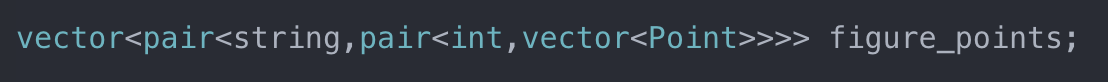
\includegraphics[scale=0.6]{optimized_struct.png}
\caption{Estrutura utilizada para armazenar conteúdo de ficheiros.}
\label{img:optimized_struct}
\end{figure}

A \textbf{string} usada representa o nome do ficheiro, o \textbf{int} representa o número de triângulos presentes no ficheiro, e o \textbf{vector<Point>} contém os pontos necessários para a figura.

O algoritmo usado, na função \textit{loadFigure} para tratar a nova estrutra foi:

\ttfamily
\begin{enumerate}
  \item Verifica se o nome do ficheiro passado como parâmetro existe na estrutura:
  \begin{enumerate}
  	\item Se sim:
	\begin{enumerate}
		\item Copia o conteúdo lá existente para a nova figura.
		\item Retorna a figura.
	\end{enumerate}
	\item Se não:
	\begin{enumerate}
		\item Lê o conteúdo do ficheiro.
		\item Coloca conteúdo na nova figura.
		\item Coloca conteúdo na estrutura para poder ser carregado posteriormente por figuras que usem o mesmo ficheiro.
		\item Retorna a figura.
	 \end{enumerate}
  \end{enumerate}

\end{enumerate}
\rmfamily



\newpage

\section{Estruturas de Dados}
\label{sec:estruturasdados}

No seguimento da fase anterior, mantivemos a estrutura geral intacta pelo que continuamos a representar o sistema solar lido do ficheiro \textbf{XML} como uma árvore, onde o primeiro nodo representa o Sol e os planetas vão ser os seus \textit{filhos}. Em consequência, as luas vão ser \textit{filhos} dos planetas e \textit{netos} do Sol. Tal estrutura pode ser vista na seguinte figura.

\begin{figure}[H]
\centering
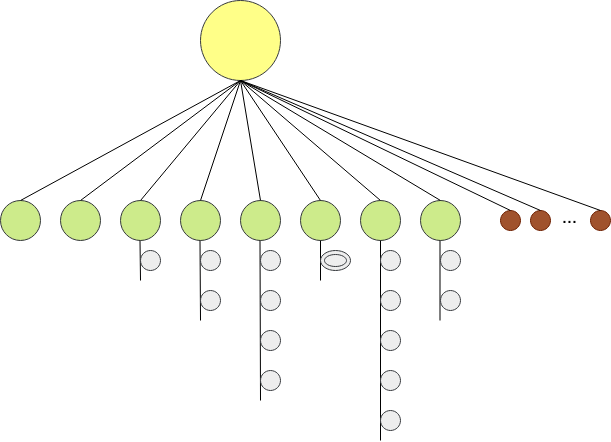
\includegraphics[scale=0.6]{tree_struct.png}
\caption{Visão geral da estrutura principal Tree.}
\label{img:tree_struct}
\end{figure}

Todas as principais classes necessárias mantiveram-se iguais à fase anterior à exceção de três, que são respetivamente a \textit{Translation}, a \textit{Rotation} e a \textit{Figure}.

\begin{figure}[H]
\centering
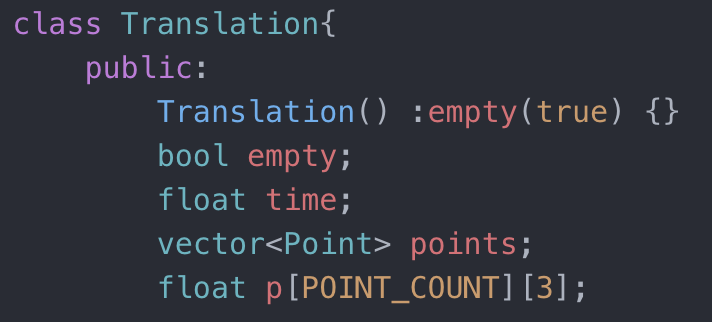
\includegraphics[scale=0.75]{translation.png}
\caption{Estrutura Translation.}
\label{img:translation}
\end{figure}

Foi necessário adicionar a variável \textbf{time} que representa o tempo que a translação vai demorar a realizar uma volta ao Sol. Foi também necessário substituir 3 variáveis que eram respetivamente \textbf{x, y, z} e representavam uma translação estática, por um \textbf{vector<Point>} que guarda os pontos de controlo necessários para a realização da curva de Catmull-Rom.

\begin{figure}[H]
\centering
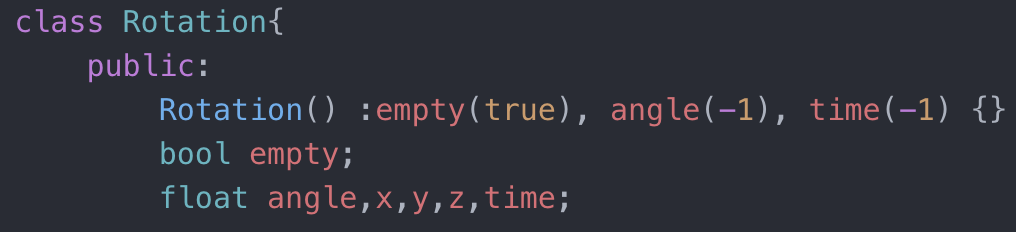
\includegraphics[scale=0.65]{rotation.png}
\caption{Estrutura Rotation.}
\label{img:rotation}
\end{figure}

Para a classe \textit{Rotation} foi necessário adicionar uma variável \textbf{time} que define o tempo que uma rotação sobre o próprio deve demorar.

\begin{figure}[H]
\centering
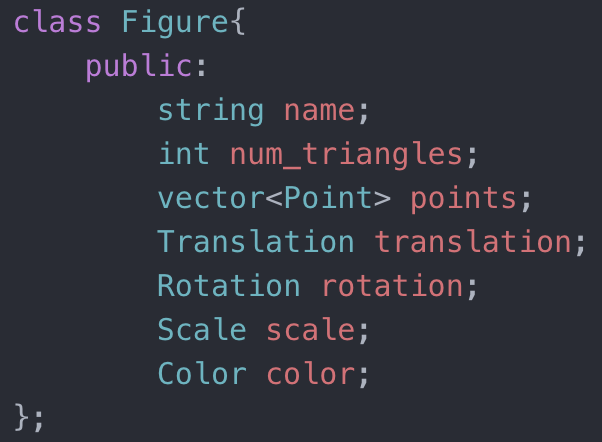
\includegraphics[scale=0.75]{figure.png}
\caption{Estrutura Figure.}
\label{img:figure}
\end{figure}

Por último à classe \textit{Figure} foi adicionada uma variável \textbf{name} que representa o nome do ficheiro que continha os pontos para que a figura fosse construída. Esta variável foi necessária para distinguir qual das figuras era o cometa (explicado mais à frente), e para uma de otimização no parsing do XML (explicado anteriormente).


\newpage

\section{Generator}
\label{sec:generator}

Para esta fase foi necessária uma evolução no \textbf{Generator}. Este tinha que ser capaz de criar um novo modelo baseado em \textbf{Patches de Bezier}.

Para proceder à realização dum modelo tendo em conta um patch de Bezier é preciso passar como parâmetro o ficheiro que contêm os pontos de controlo  \textbf{(patch)}, o nível de \textbf{tessellation} e por último o \textbf{nome do ficheiro} onde será guardado o resultado.

\begin{figure}[H]
\centering

\includegraphics[scale=0.75]{bezier_command.png}
\caption{Exemplo de invocação.}
\label{img:bezier_command}
\end{figure}

O resultado que será guardado em ficheiro serão todos os pontos necessários para a criação dos triângulos que posteriormente modelam a superfície cúbica.

\subsection{Algoritmo de geração do modelo}
\label{sec:bezier}

O algoritmo desenvolvido divide-se em 3 partes essenciais. A primeira é o \textbf{parsing do patch}, a segunda é a \textbf{criação da superfície de Bezier} que necessita da terceira parte que é o \textbf{cálculo dos pontos} da superfície.

\subsubsection{Parsing do Patch}

Para a fase parsing do patch tivemos em conta o habitual formato destes patchs, descrito na seguinte imagem.

\begin{figure}[H]
\centering
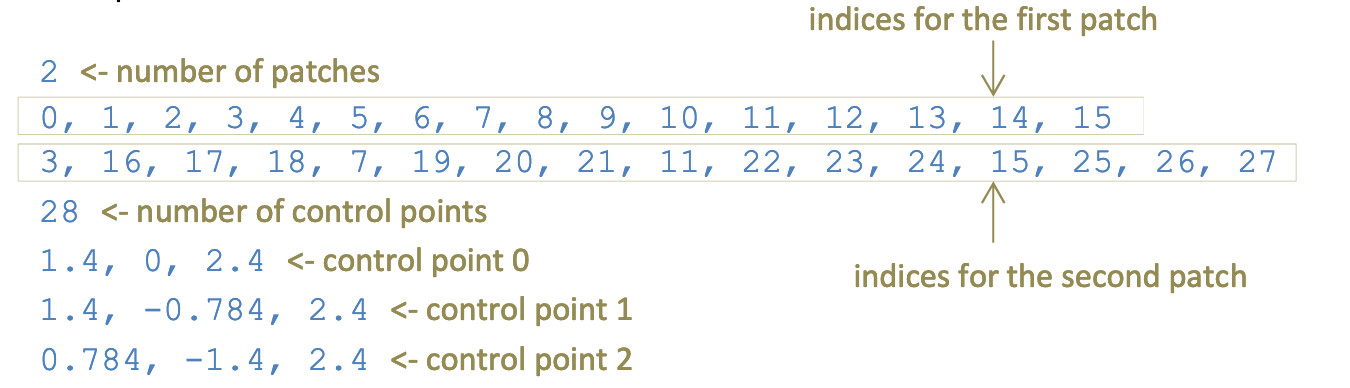
\includegraphics[scale=0.60]{patch_format.png}
\caption{Exemplo dum formato dum patch.}
\label{img:bezier_command}
\end{figure}

O algoritmo utilizado para fazer parsing ao ficheiro foi:

\ttfamily
\begin{enumerate}
  \item Abre o ficheiro (patch) passado como parâmetro.
  \item Lê a primeira linha (number os patches) e cria um array que irá conter cada patch (patches).
  \item Realiza ciclo de leitura dos patches e armazena-os no array patches.
  \item Lê linha seguinte aos patches que representa o número de pontos de controlo (number\_control\_points).
  \item Realiza ciclo de leitura dos pontos, e coloca-los no array control\_points.
\end{enumerate}
\rmfamily


\subsubsection{Criação da Superfície de Bezier}

Para criar a superfície de Bezier é preciso ter em conta a função de parsing apresentada anteriormente, e ainda a função de cálculo dum ponto que está presente na subsecção seguinte.

O algoritmo utilizado para a criação da superfície foi:

\ttfamily
\begin{enumerate}
  \item Faz parsing do ficheiro (patch).
  \item Para cada patch existente (patch\_number):
  \begin{enumerate}
  	\item Para todos os níveis de tessellation (tessellation\_v) entre 0 e tessellation, calcula-se:
	\vspace{0.5cm}

	\hspace{0.0cm} $$v = \frac{tessellation\_v}{tessellation}$$

	\vspace{0.5cm}

	\begin{enumerate}
		\item Para todos os níveis de tessellation (tessellation\_u) entre 0 e tessellation, calcula-se:
		\vspace{0.5cm}

		\hspace{0.0cm} $$u = \frac{tessellation\_u}{tessellation}$$

		\vspace{0.5cm}
		\item Calculam-se os dois triângulos necessários, recorrendo ao algoritmo apresentado na subsecção seguinte (Cálculo dum Ponto):
		\vspace{0.3cm}

      		\underline{Primeiro triângulo:}

     		\vspace{0.3cm}

          	P1 $\Rightarrow$ (patch\_number, u, v)

      		\vspace{0.2cm}

          	P2 $\Rightarrow$ (patch\_number, u + $\frac{1}{tessellation}$, v)

      		\vspace{0.2cm}

         	P3 $\Rightarrow$ (patch\_number, u + $\frac{1}{tessellation}$, v + $\frac{1}{tessellation}$)

      		\vspace{0.3cm}

		\underline{Segundo triângulo:}

      		\vspace{0.3cm}

          	P1 $\Rightarrow$ (patch\_number, u + $\frac{1}{tessellation}$, v + $\frac{1}{tessellation}$)

      		\vspace{0.2cm}

          	P2 $\Rightarrow$ (patch\_number, u, v + $\frac{1}{tessellation}$)

      		\vspace{0.2cm}

          	P3 $\Rightarrow$ (patch\_number, u, v)

      		\vspace{0.2cm}

	\end{enumerate}
  \end{enumerate}
  \item Escreve resultados em ficheiro.
  \item Limpa memória.
\end{enumerate}
\rmfamily


\newpage

\subsubsection{Cálculo dum Ponto}

Para que um ponto da superfície de Bezier seja calculado é necessário que sejam passados como parâmetros, o \textbf{número do patch} em que este se encontra, os pontos calculados anteriormente que se ligam à tessellation, \textbf{u} e \textbf{v}.

O algoritmo para o cálculo dum ponto foi:

\ttfamily
\begin{enumerate}
  \item Criámos 2 arrays, um para u e outro para v, e em cada índice dos arrays residem \textbf{polinómios de Bernstein} que têm em conta o índice em questão.
  \vspace{0.5cm}

  \hspace{0.0cm} $$B_{i} = t^i (t-1)^{3-i} \binom{3}{i}  , \forall i \in \{0,4\}, t \in \{u,v\}$$

  \vspace{0.5cm}

  \hspace{-2.8cm}bpu[4] = \{ powf(1-u, 3), 3*u*powf(1-u, 2), 3*powf(u, 2)*(1 - u), powf(u, 3) \};

  \vspace{0.5cm}

  \hspace{-2.8cm}bpv[4] = \{ powf(1-v, 3), 3*v*powf(1-v, 2), 3*powf(v, 2)*(1 - v), powf(v, 3) \};

  \vspace{0.5cm}

  \item Para cada índice de bpu:
  \begin{enumerate}
  	\item Para cada índice de bpv:
	\begin{enumerate}
		\item Calcula o índice do patch a ser usado.
		\item Calcula o índice do ponto de controlo utilizando o índice calculado anteriormente.
		\item Para cada coordenada do ponto a ser calculado, adiciona-se a multiplicação do respetivo ponto de controlo com os polinómios de Bernstein correspondentes a u e v.
	\end{enumerate}
  \end{enumerate}
  \item Retorna o ponto a ser usado para a criação da superfície.
\end{enumerate}
\rmfamily



\newpage

\section{Engine}
\label{sec:engine}

\subsection{Catmull-Rom Cubic Curves}
\label{sec:catmullrom}


\newpage

\subsection{VBOs}
\label{sec:vbos}

Nesta fase é requerido que os modelos sejam desenhados com VBOs, ao invês do que acontecia nas fases anteriores.

Para tal, no momento do desenho das figuras é realizado o seguinte processo:

\ttfamily
\begin{enumerate}
  \item Geração de um \textit{Vertex Buffer Objects};
  \item Especificação do objeto associado ao VBO gerado $\Rightarrow$ \textit{GL\_ARRAY\_BUFFER}
  \item Alocação de memória para um array de floats \textbf{v} com o espaço necessário para os pontos da figura:
    \begin{itemize}
      \item sizeof(float) $\times$ num\_triangles $\times$ 3 (num\_vertices) $\times$ 3 (num\_coordinates)
    \end{itemize}
  \item Ciclo de carregamento dos pontos da estrutura de dados para o array de floats:
    \begin{itemize}
      \item v[i++] = it->x;
      \item v[i++] = it->y;
      \item v[i++] = it->z;
    \end{itemize}
  \item Preenchimento do \textit{GL\_ARRAY\_BUFFER} com os pontos do array \textbf{v};
  \item Transformação num array de vértices;
  \item Desenho dos triângulos com base no array processado.
\end{enumerate}
\rmfamily


\newpage

\section{Scenes}
\label{sec:scenes}

Nesta fase do projeto é requerido um modelo dinâmico do sistema solar, com o sol, os planetas e os satélites naturais do mesmo. Além disso, o sistema solar deve incluir também um cometa com uma trajetória definida através duma curva de Catmull-Rom. Este cometa deve ser criado tendo por base os pontos de controlo do \textbf{Patch de Bezier} correspondente ao \textit{teapot}. Desta forma o cometa terá, inevitavelmente, a forma dum \textit{teapot}.

De seguida, nas figuras \ref{img:scene_1} e \ref{img:scene_2}, são disponibilizados exemplos estáticos do sistema solar, onde é possível verificar a presença de todos os objetos requisitados.

\begin{figure}[H]
\centering
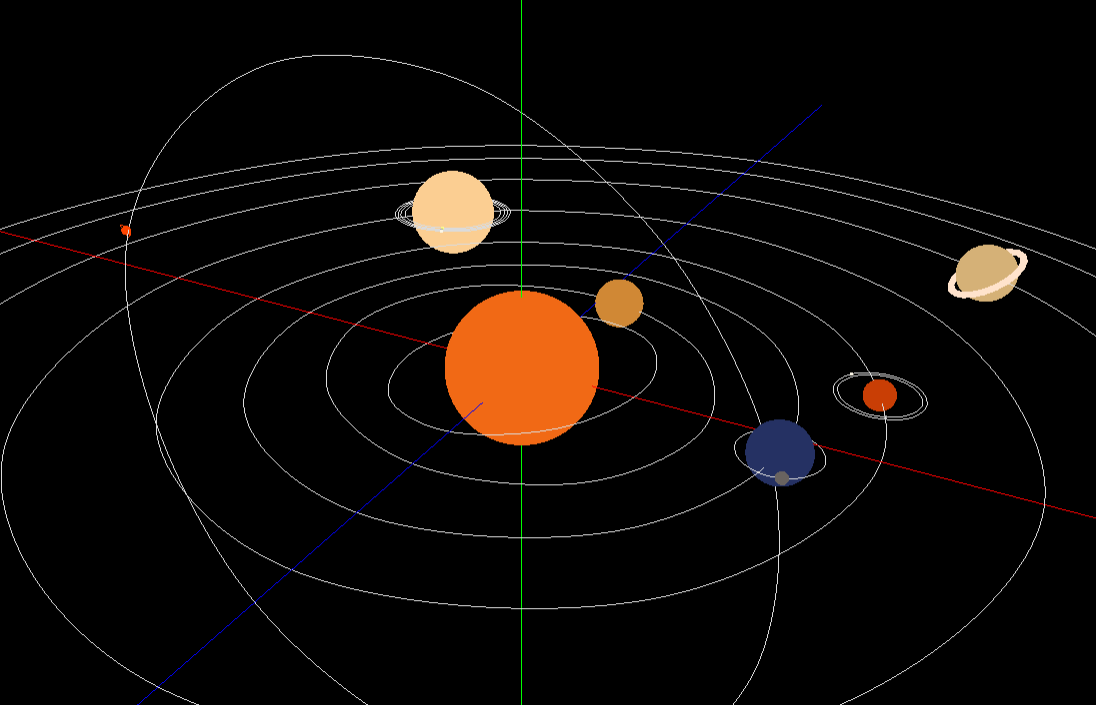
\includegraphics[scale=0.3]{scene_1.png}
\caption{Possível perspetiva da cena.}
\label{img:scene_1}
\end{figure}

\begin{figure}[H]
\centering
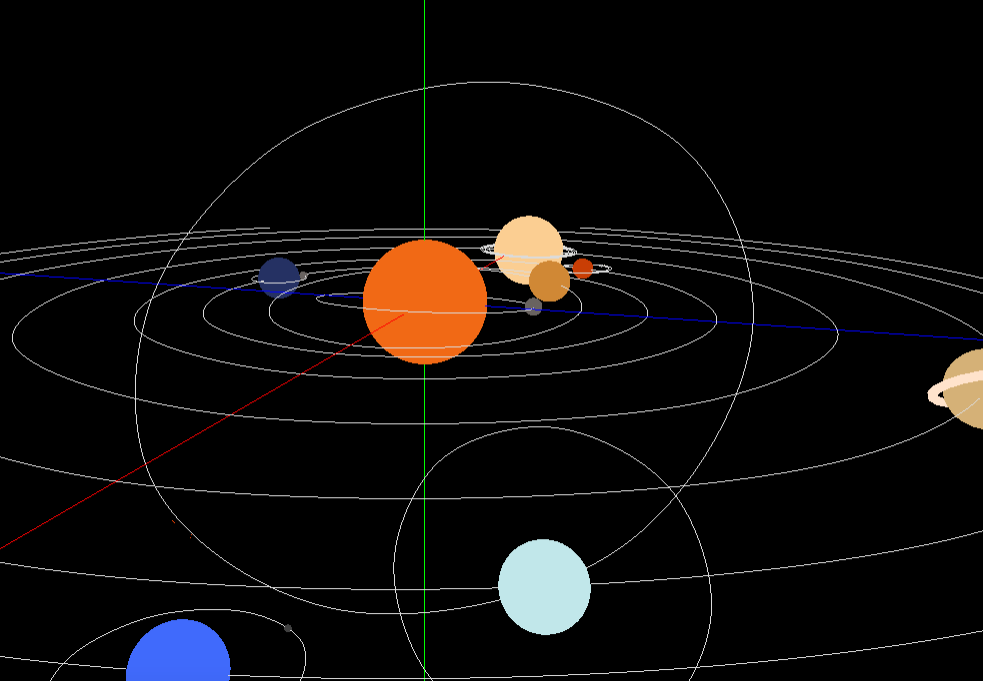
\includegraphics[scale=0.36]{scene_2.png}
\caption{Possível perspetiva da cena.}
\label{img:scene_2}
\end{figure}


\section{Conclusão}
\label{sec:conclusao}


\section{Bibliografia}
\label{sec:bibliografia}


\end{document}
